\subsubsection{How are the security and performance is ensured in a product of a company?}
\label{security_performance}

To identify general practices among the Bangladesh software industry regarding software products' security and performance, we have included two open-ended questions in the survey. This particular question covers how a company secures its code from external attack and maintain its performance after deployment. However, the performance of a software product is related to the scalability of the solution. So, we will cover the following points here:
\begin{itemize}
    \item Security
    \item Performance
    \item Scalability
\end{itemize}


\paragraph{Security:}
\label{Security}

\begin{figure}[h]
\centering
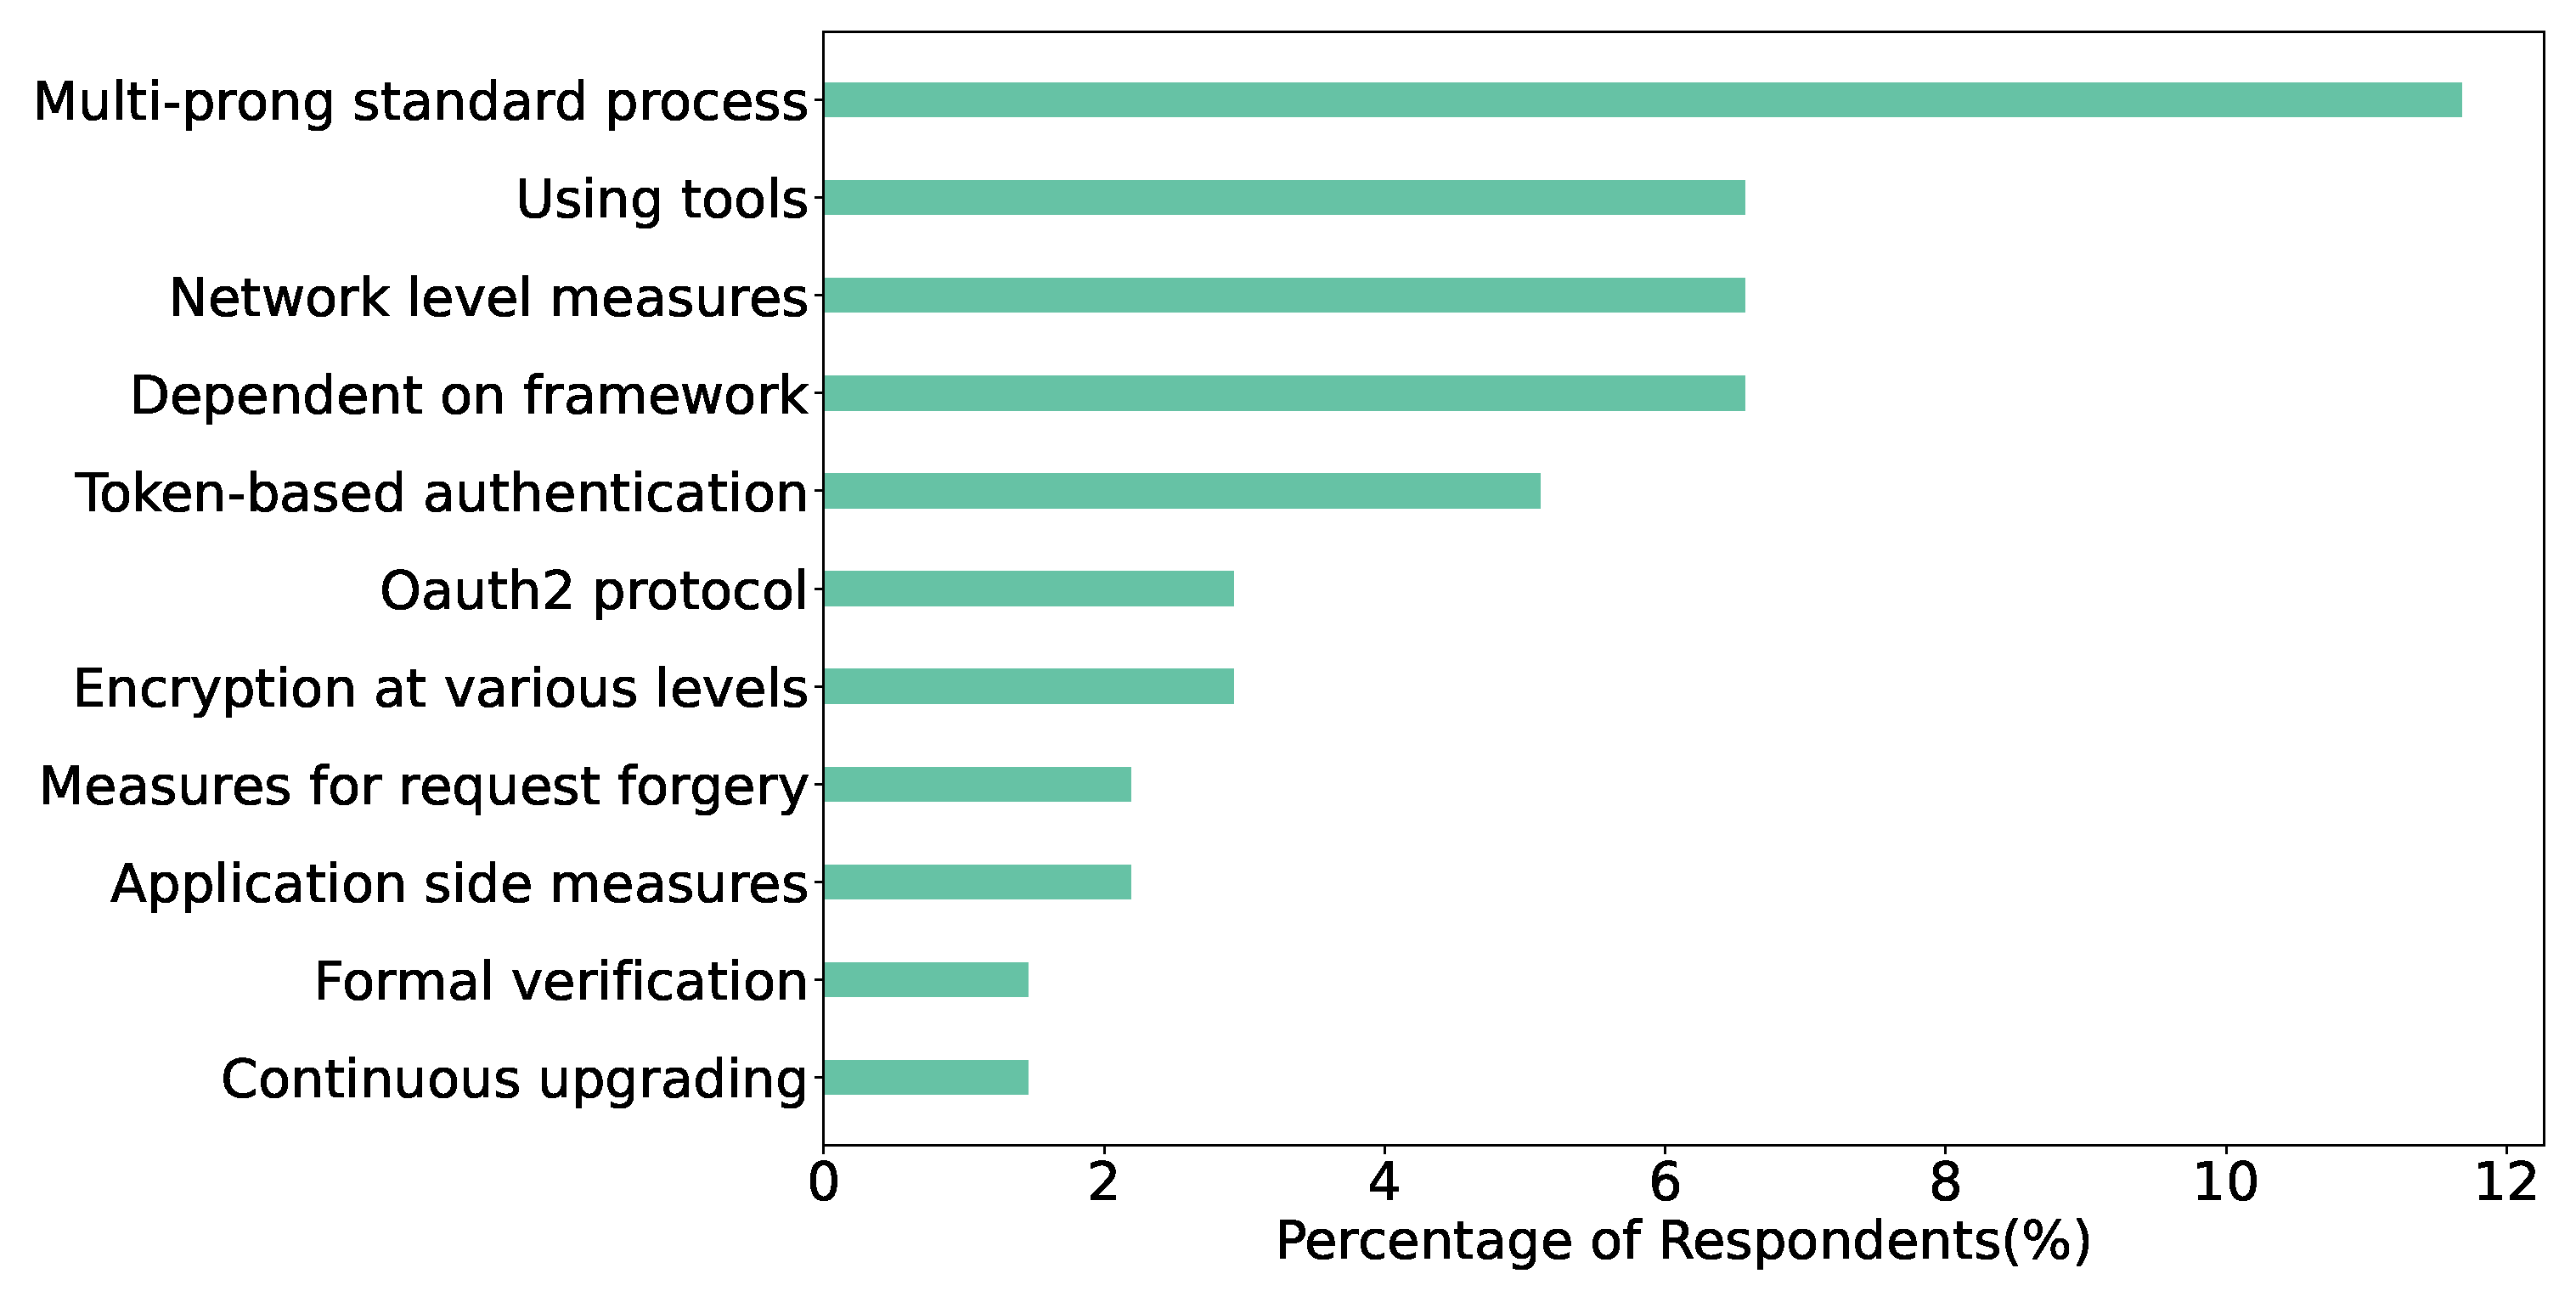
\includegraphics[scale=0.22]{Figures/Security.eps} 
\caption{Measures to ensure security of products}
\label{fig:Measures to ensure security}
\end{figure}


Authentication and authorization-based security are the most prominent practice in the Bangladesh software industry to ensure software products' security. The other categories are security based on framework/platform/tools and encryption. Under these categories, several measures are usually followed. Security measures of Bangladesh SE industry is presented in Figure \ref{fig:Measures to ensure security}. The measures of the each categories are discussed below,

Measures under the \emph{authentication and authorization} category is practised by 25.55\% respondents to ensure security. The measures are 
\begin{enumerate}[label=(\alph*)]

    \item \textbf{Multi-prong Standard Process} : About 11.68\% of the total respondents reported that they practices various security standard and protocol to ensure security. The standard includes ISO/IEC 27001 , and PA DSS
    \surveyquote{Multi Prong Standard Processes and Products}{110}
    
    \item \textbf{Token-based authentication} : A token-based authentication system allows users to enter their username and password to obtain a token, which allows them to fetch a specific resource - without using their username and password. Once their token has been obtained, the user can offer the token, which offers access to a specific resource for a time period - to the remote site. 5.11\% of people expressed its eligibility.
    \surveyquote{Token based authentication for all of my rest service}{80}
    
    \item \textbf{OAuth 2.0} : OAuth 2.0 is the industry-standard protocol for authorization. OAuth 2.0 focuses on client developer simplicity while providing specific authorization flows for web applications, desktop applications, mobile phones, and living room devices. Many (2.92\%) respondents use the OAuth 2.0 protocol as the main way of maintaining security.
    \surveyquote{OAuth 2.0, JWT, Token Base Authentication, CORS Filter, XSRF}{127}
    
    \item \textbf{Application Side Measures}: 2.19\% of respondents responded that they implement security measures at the application level. This measure includes encryption of application data at the client-side, use of https while pulling data from a server, secured architecture etc.
    \surveyquote{At application level, could not achieve others yet}{72}
    
    \item \textbf{Measures for request forgery}: Measures against cross-site forgery are implemented to ensure security. This includes CORS or cross-origin resource sharing, CSRF, or cross-site request forgery or one-click attack or XSRF. 2.19\% of respondents implemented measures against  Cross-site request forgery to ensure security.
    \surveyquote{Security testings like: SQL injection, cross-site scripting, CSRF, API security, use of https,  detecting malicious / suspicious HTTP requests and auto-blocking}{42}
    
    \item \textbf{Formal Verification}: A code-level review can mitigate security threats. 1.46\% respondents ensured the practice of formal code review.
    \surveyquote{There are some basic guidelines that we must follow and while code review this needs to be an absolute part that needs to be checked before the code gets merged}{112}
    
\end{enumerate}

21.17\% respondents use several technology, tools,platform to ensure security of their product. Measures under the \emph{framework/platform/tools} category are,
\begin{enumerate}[label=(\alph*)]

     \item \textbf{Dependent on Framework} : The common frameworks provide basic to intermediate level security measures in the application. 6.57\% of respondents depend on the framework for security. The framework includes popular frameworks such as spring and  HDIV. We have found that respondents using Spring and Laravel framework mostly reported depending on the framework for security. However, the observation is not statistically significant.
    \surveyquote{https, popular framework which already prevents some type of attacks. rest of the things on case-by-case basis)}{79}
    
    \item \textbf{Use of tools} : Respondents use various open-source/ paid tools for scanning and testing. These tools help to find security threats in an existing system. The tools include OWASP based tools and  penetration testing tools.
    \surveyquote{use encryption at different level of software (server, network, transmission layer, database and software layer.)}{35}
    
    \item \textbf{Network level Measures}: Network-level measures include IP-white-listing, port-blocking, VPN, and use of HTTPS  in software. 6.57\% of respondents use at least one of the before-mentioned strategies to ensure security.
    \surveyquote{network blocking and common security measures}{2}

    \item \textbf{Continuous Upgrading}: As security threats are evolving; thus, current systems need continuous up-gradation in a frequent interval. 1.46\% of respondents said they arrange frequent hackathons, workshops, and security audits to address the continuously evolving security threat.
    \surveyquote{We run security audit of our office environment. We also conduct security session per 6 months to introduce latest trend in threats and what we can do to avoid it}{57}

\end{enumerate}

2.92\% of respondents use encryption technologies to encrypt their data. Respondents use encryption at the different levels of software architecture such as network, data, transmission, and ensure their security.
\surveyquote{use encryption at different level of software (server, network, transmission layer, database and software layer.)}{35}
\boxtext{Security testing and the use of security standards are prevalent in the Bangladesh SE industry.}


% To maintain security of software product SE industry of Bangladesh is mainly dependent on standard process which includes cloud based security, third party software, OS hardening followed by uses of security tools, network level measures and framework security. As found by Harrison et al.\cite{Harrison2010} network level measures are the first choice in ensuring security of software product which matches with our findings. Srinivasan et al.\cite{Srinivasan2017} listed top 10 web framework in terms of security testing where Spring framework achieved 7\textsuperscript{th} position. From figure ~\ref{fig:frameworks} we have seen that most of our respondents use Spring framework for software development. This might be the reason that a lot number of respondents dependent on framework for ensuring security.


\paragraph{Performance}
\label{Performance}

\begin{figure}[h]
\centering
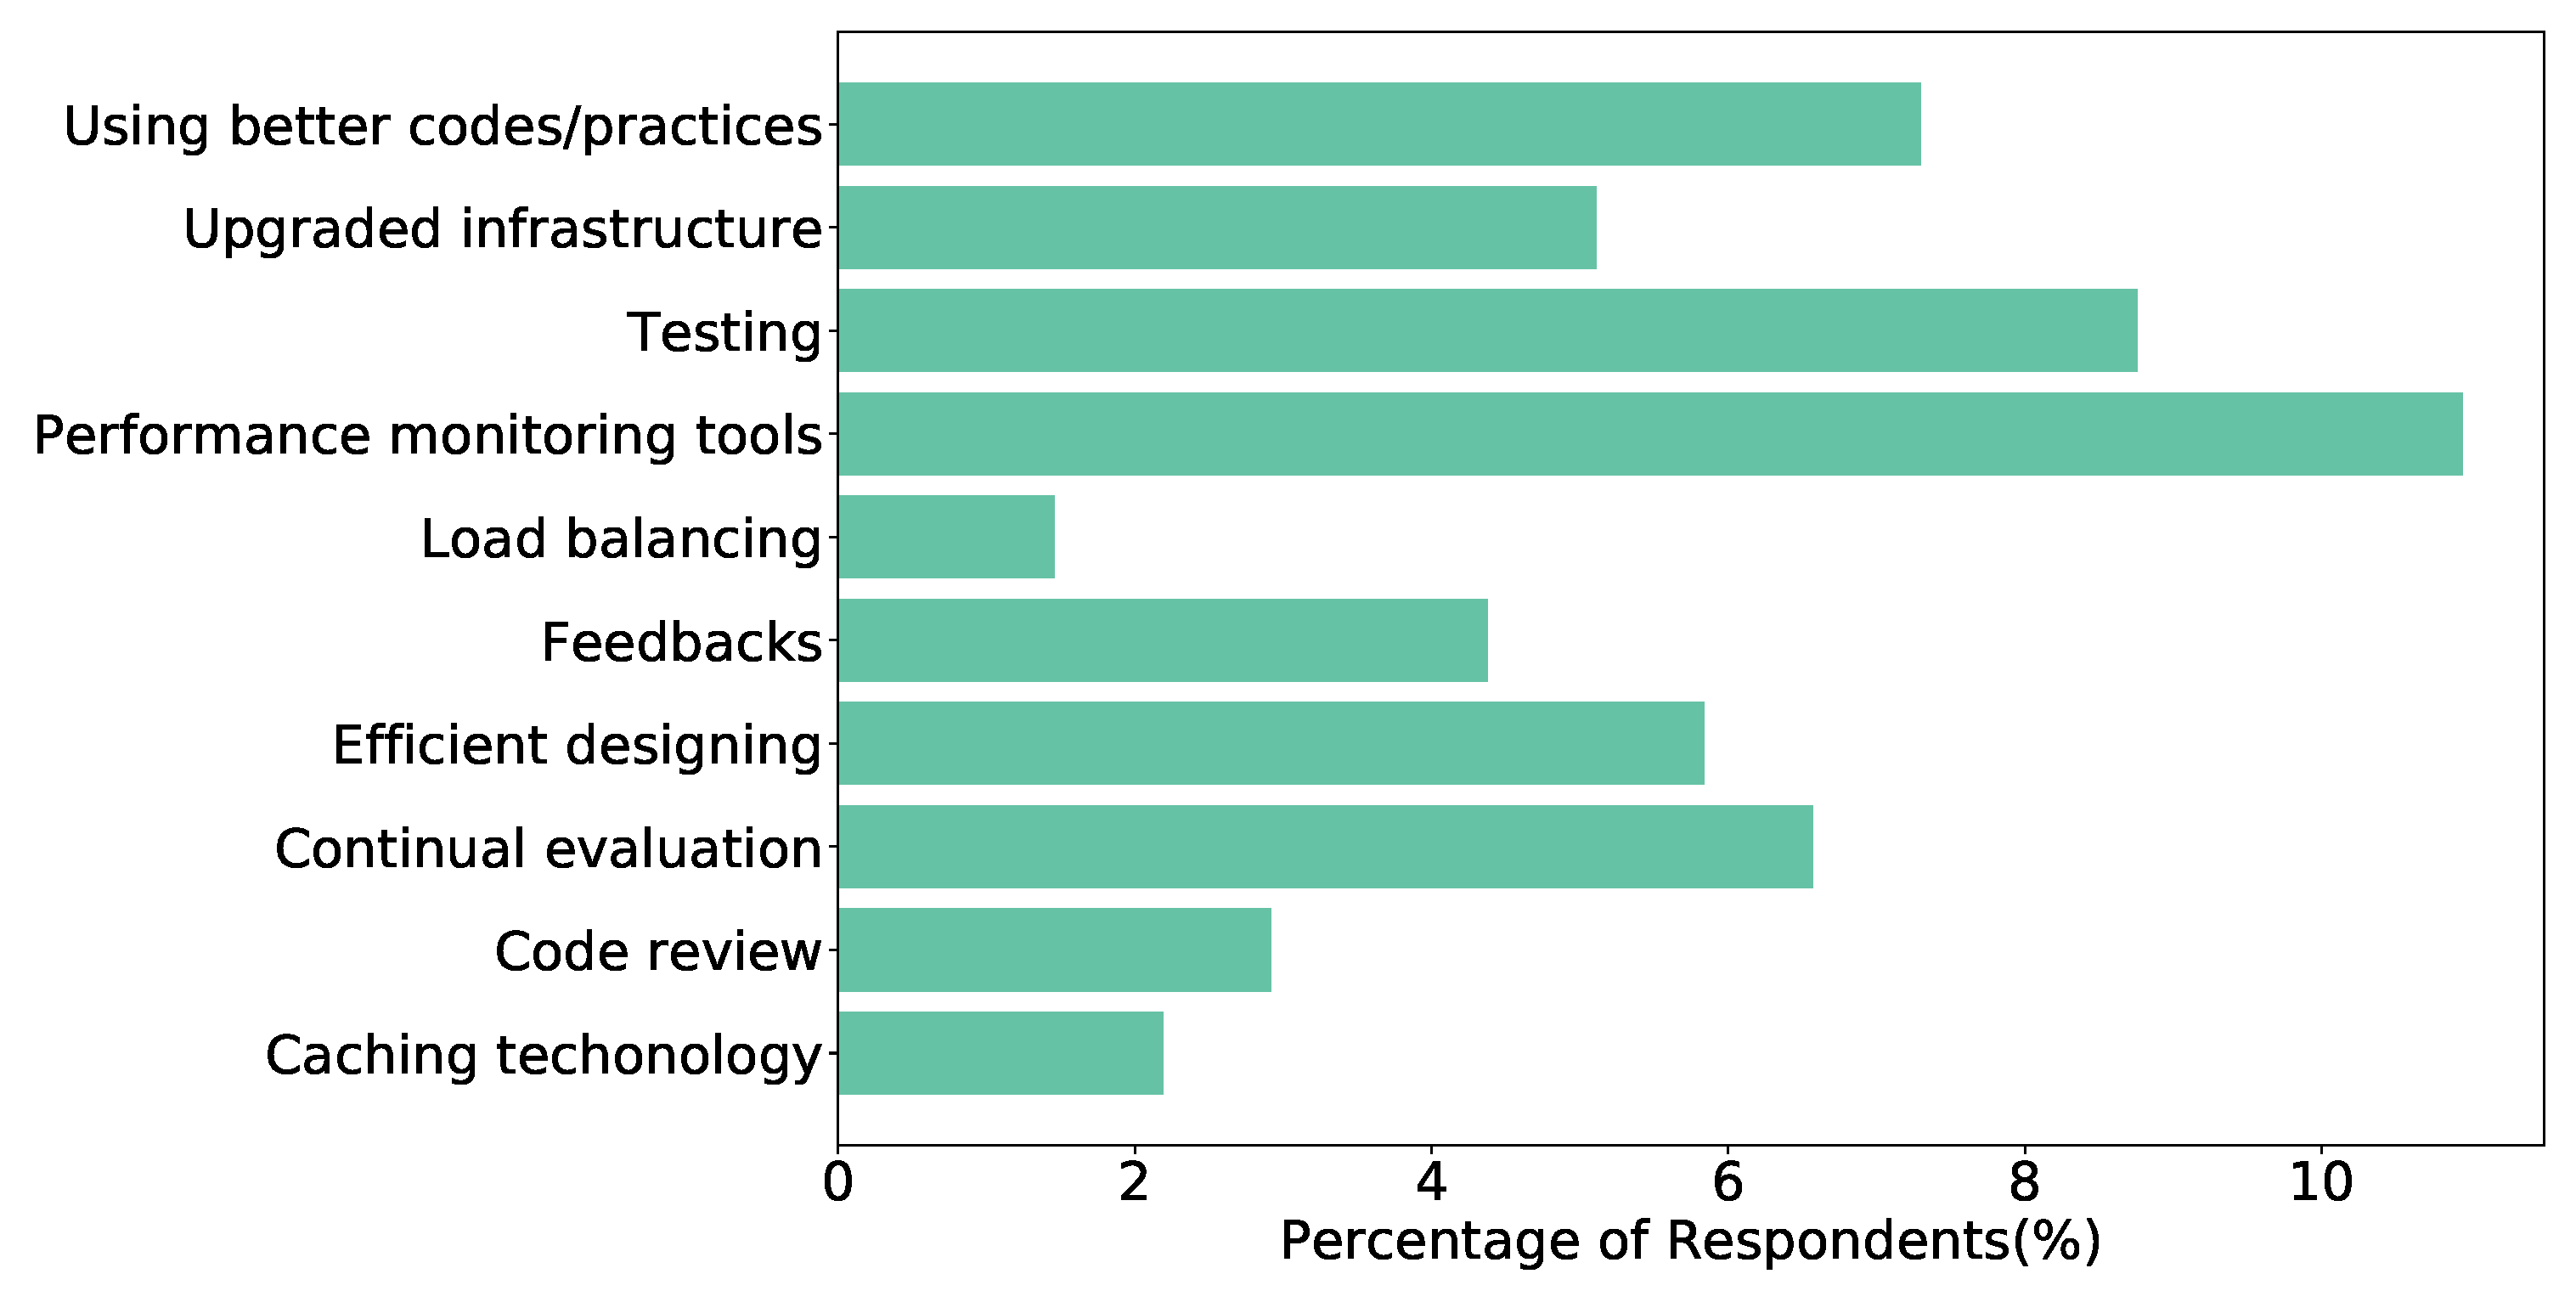
\includegraphics[scale=0.22]{Figures/Performance.eps} 
\caption{Measures to ensure performance of products}
\label{fig:Measures to ensure performance}
\end{figure}

Software performance indicates how efficient the software is in terms of resources and time. Use of framework/tools/platform to ensure software performance is a dominant practice in the Bangladesh SE industry. The other type of practices are peer-review, software design, and software testing. Respondents in our survey reported multiple measures under these categories.
The measures are presented in Figure \ref{fig:Measures to ensure performance}. The measures in \emph{framework/tools/platform} category are,
\begin{enumerate}[label=(\alph*)]

    
    \item \textbf{Performance Monitoring Tools}: There are various performance monitoring automated tools from which we can measure the overall and component-wise performance. 14.6\% of respondents use these tools to measure performance. Respondents use several performance metrics such as error/crash rate, response time, uptime, etc.
    \surveyquote{take help of different performance monitoring tools and dashboard, analyzed data , measure time and memory efficiency of process}{35}
    
    \item \textbf{Upgraded Infrastructure}: 5.11\% of respondents use upgraded infrastructure to ensure performance. This infrastructure includes cloud hosting, a high-end server, and new technologies.
    \surveyquote{Amazon Hosting and Quality Software}{85}
    
    \item \textbf{Caching Technology}: Caching mechanism improves performance by reducing response time. 2.19\% of respondents rely on caching to maintain software performance.
    \surveyquote{... Good Caching}{29}
    
    \item \textbf{Load Balancing}: Load balancing can improve the system performance by ensuring an equal load to all servers. 1.46\% of respondents think of using load balancing as a measure to maintain performance.
    \surveyquote{Optimizing number of HTTP requests, Asynchronous programming, Caching, CDN, Load Balancing, nginx, varnish, compression of data, Continuous monitoring, Load testing, stress testing}{42}

\end{enumerate}


13.14\% of respondents ensure software performance  at design phase. Measures of this category are,

\begin{enumerate}[label=(\alph*)]

    \item \textbf{Using better codes/practices}: Industry-standard best practices can improve system performance. 7.3\%respondents ensure performance by implementing best practices. The best practices include compression technology, enforcing design patterns, and refactoring.
    \surveyquote{Implementation time carefulness and maintaining a well developed coding standard}{40}
    
    \item \textbf{Efficient designing}: Software performance is dependent on the architecture of the system. 5.84\% of respondents emphasize design to ensure performance.
    \surveyquote{By careful designing}{24}

\end{enumerate}

 8.76\% of respondents of our survey rely on the software testing strategy to ensure performance. Performance is ensured by various rigorous testing phase. The phase includes load testing, stress testing, integration testing.
 \surveyquote{By rigorous testing and checking performance testing}{17}
 
 Reviewing peer and user, tester feedback can be a good strategy to ensure performance. 7.3\% of our respondents use measures from this category to ensure performance. Measures under this category are,
 
 \begin{enumerate}[label=(\alph*)]
 
     \item \textbf{User Feedback}: It is a great source of performance measure. Taking time to time feedback from the clients helps a company realize how their products are performing. Many (4.38\%) respondents have highly recommended it.
    \surveyquote{Continuous feedback from clients and QA team}{65}
    
    \item \textbf{Code Review}: About 2.92\% of people have said that a proper and attentive code review can reduce the codes' faults and, therefore, enhance the performance of a software.
    \surveyquote{The code quality is assessed by the different team members during code review, followed by designing new ways to solve issues in the product that are time-intensive.}{15}
 
 \end{enumerate}
\boxtext{For performance, the Bangladesh SE industry is largely dependent on monitoring tools and software testing.}


\paragraph{Scalability}
\label{Scalability}
\begin{figure}[h]
\centering
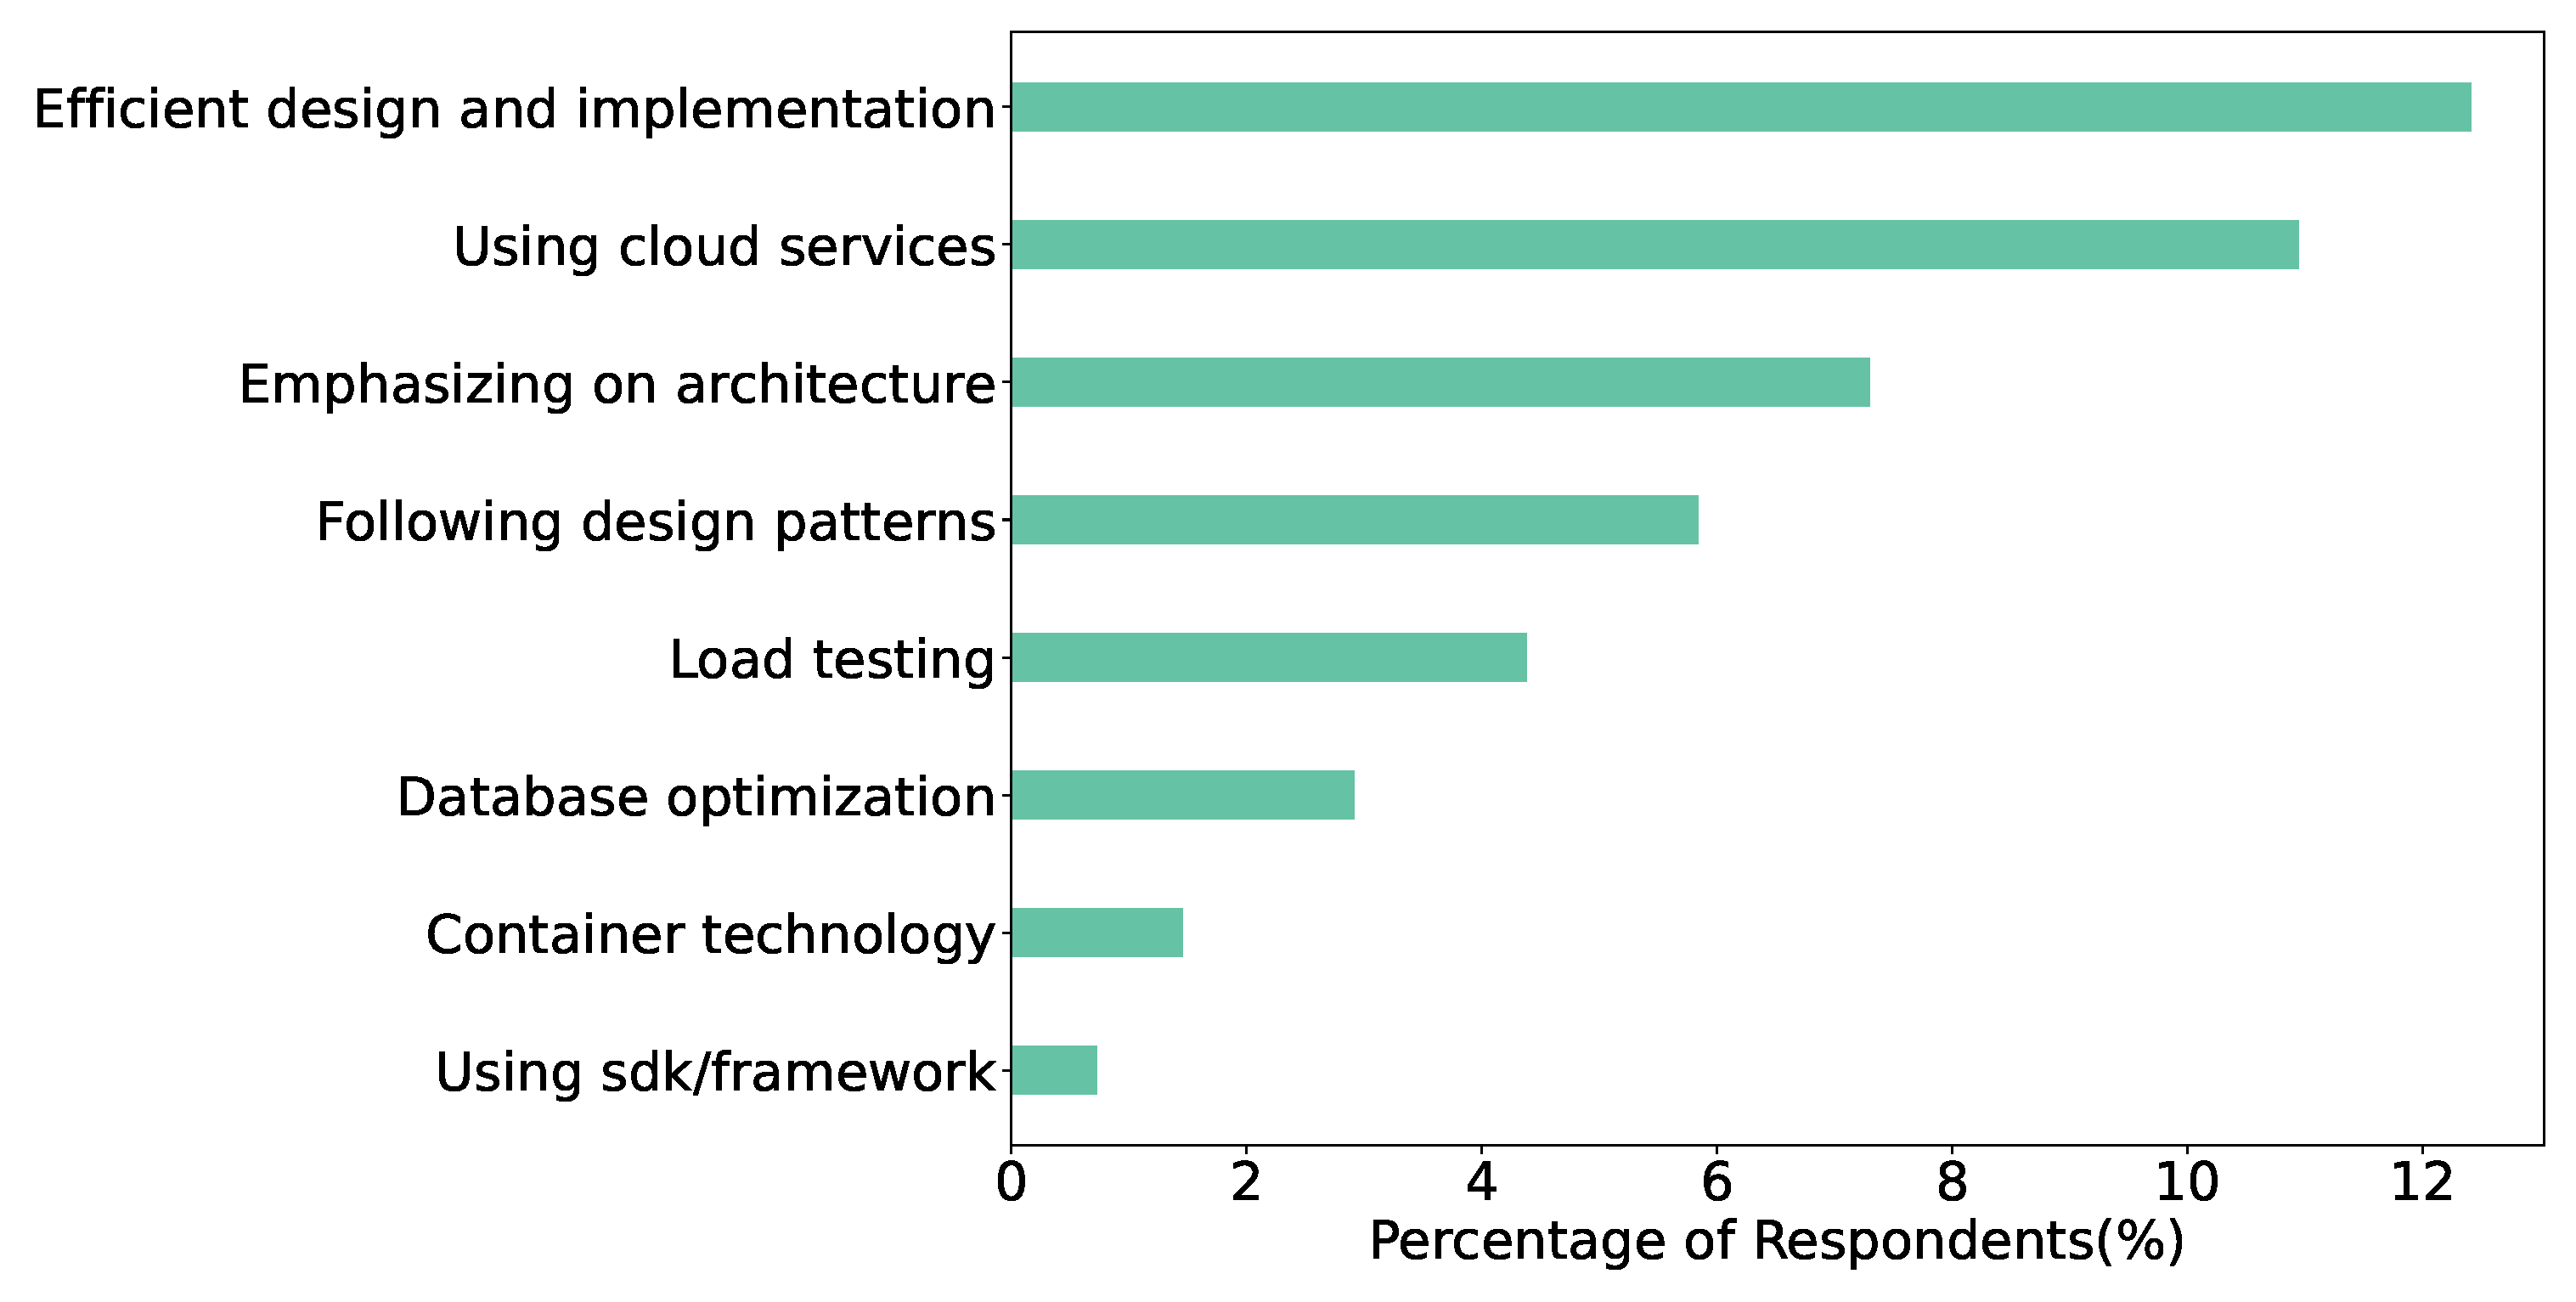
\includegraphics[scale=0.22]{Figures/Scalability.eps} 
\caption{Measures to ensure scalability of products}
\label{fig:Measures to ensure scalability}
\end{figure}


 Software scalability defines the ability to scale up a solution. Issues with little importance can impede scaling up. Thus proper measures should be taken from the design stage to ensure the scalability of the system. Scalability ensured by efficient software design is the most practices strategy in the Bangladesh SE industry. 25.55\% reported using at least one of the measures in this category. The measures practices in Bangladesh SE industry are presented in Figure \ref{fig:Measures to ensure scalability}. The measures in \emph{efficient software design} category are,
% Recent days the cloud services offer tools to accomodate custom reactive scaling strategies. Thus, it has become easier to ensure scalability using cloud services \cite{Falatah2014}. Our results  also follows the world trend, usage of cloud services has placed 2\textsuperscript{nd} in terms popularity of scalability measures in SE industry of Bangladesh.
 \begin{enumerate}[label=(\alph*)]
 
     \item \textbf{Efficient Design and Implementation}: 12.41\% of respondents emphasize on the design and implementation of a scalable architecture. 
    \surveyquote{During implementation we always keep in mind about the scaling factor}{40}
    
     \item \textbf{Emphasizing on architecture}: 7.3\% of respondents emphasized on architecture. It is mostly micro-service architecture which they use to ensure scalability.
    \surveyquote{We follow the micro-service architecture. In a nutshell, we scale up the module vertically which is necessary. We use docker along with Jenkins for automatic deployments and scaling.}{10}

    
    \item \textbf{Following Design Patterns}: Some design patterns inherently help in the time of scaling. 5.84\% of respondents think that following these design patterns will be of great use for software scalability.
    \surveyquote{Following certain design patterns}{8}
 
 \end{enumerate}
 
 13.14\% of respondents of our survey use framework or some kind of tool to ensure scalability. The measures in this category are,
\begin{enumerate}[label=(\alph*)]

    \item \textbf{Using Cloud Services}: 10.95\% user depends on cloud services like AWS and Azure for the scalability of the system. Modern features like elastic load balancing and auto-scaling make it easy to ensure scalability.
    \surveyquote{Using AWS Elastic Load Balancer}{28}
    
    \item \textbf{Container Technology}: Container technologies include Docker, Kubernetes, which ensure OS-level virtualization. By standardizing the system, container technologies ease the scaling of an infrastructure.1.46\% of respondents use these measures to ensure product scalability. Containers enable users to scale their system without any worries about the underlying OS.
    \surveyquote{We used Docker technology}{85}
    
    \item \textbf{Using SDK/framework}: Modern frameworks ensure scalability by default. 0.73\% of respondents solely depend on the framework for scalability.
    \surveyquote{following flexible framework which allows better scalability}{14}
  
\end{enumerate}
 
 
There is one measure under the software testing category, which is load testing. Load testing can be used to check the scalability of a system. 4.38\% of respondents use load tests to check whether their system is scalable or not.
\surveyquote{through load testing and load simulation.}{35}

There is also one measure under the Database Design category, which is database optimization. Database optimization includes sharding, clustering, indexing, and scaling. 2.92\% of respondents optimize database to scale their system.
\surveyquote{Besides scaling horizontally, database scaling is performed by partitioning tables, along with multi-threaded implementations}{85}
\boxtext{Typically software scalability is considered at the design phase in the Bangladesh SE industry.}
\boxtext{The use of cloud services is one of the common measures to ensure scalability.}